\chapter{Anhang}
\begin{table}[h]
    \centering
    \caption[Messtechnisch ermittelte Flussdichten]{Im Luftspalt gemessene Flussdichten $B$ bei verschiedenen Spulenströmen.}
    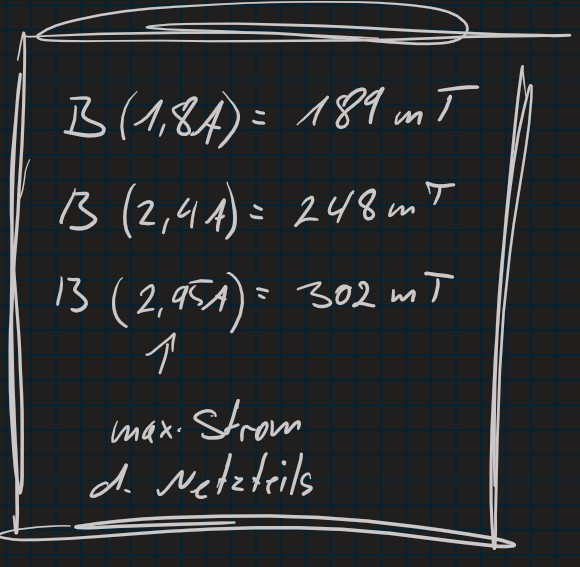
\includegraphics[height=.5\textheight]{messungen/messungen_flussdichte.jpg}
    \label{tab:messwerte_flussdichte}
\end{table}

\begin{table}[h]
    \centering
    \caption[Messwertetabelle]{Messwerte für \textsc{Hall}-Spannungen $U_H$ und Probenspannungen $U_p$ bei verschiedenen Probenströmen $I_p$ mit dem Spulenstrom $I_S$ als Parameter.}
    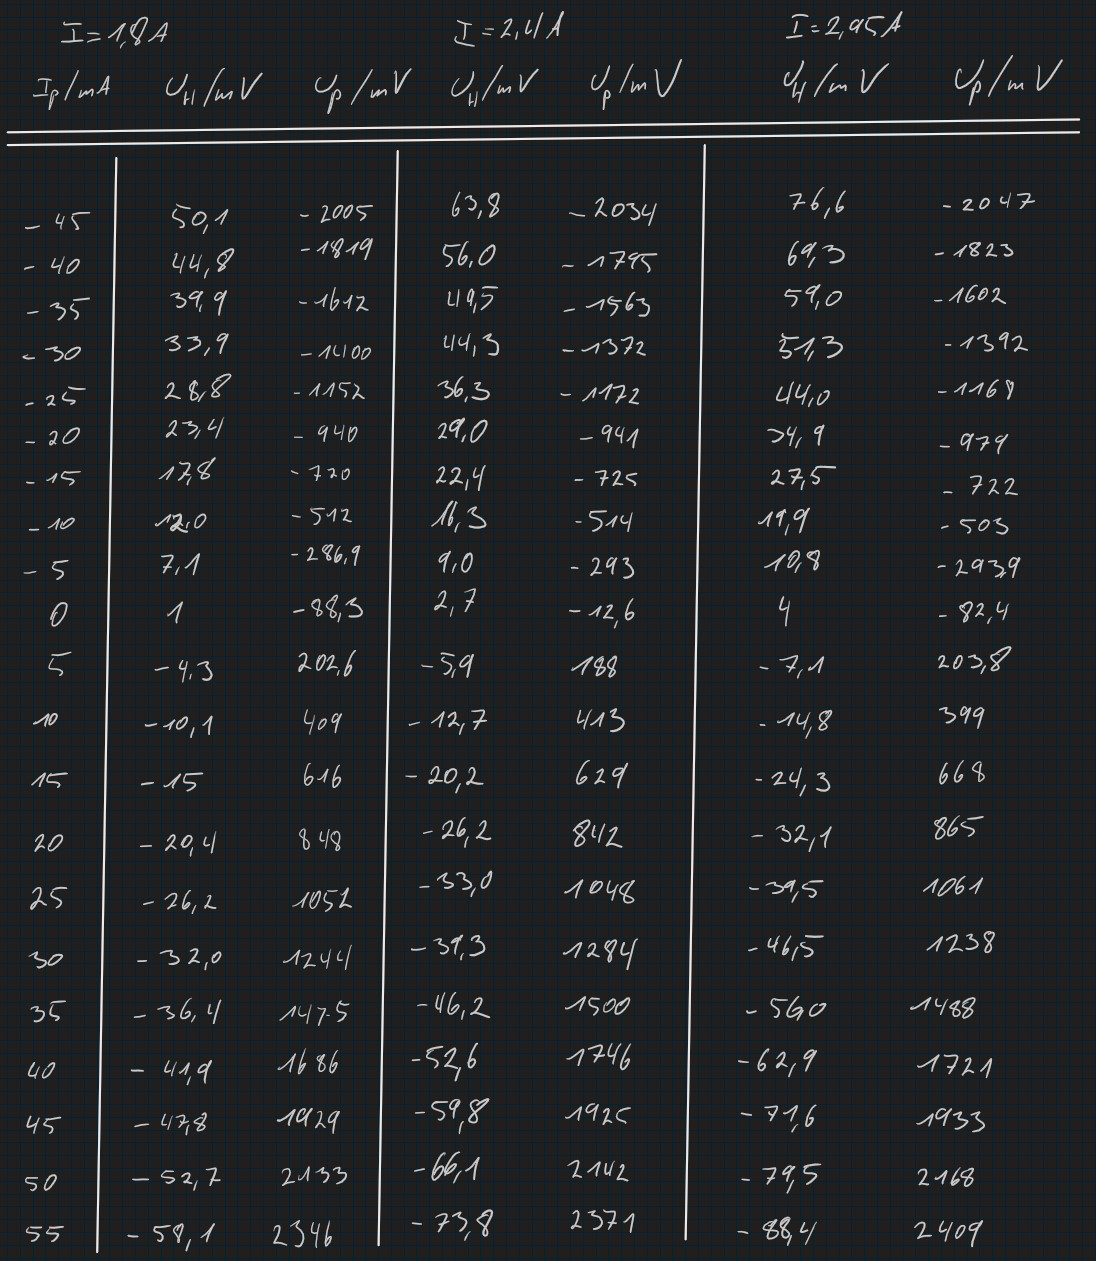
\includegraphics[height=.8\textheight]{messungen/messungen.jpg}
    \label{tab:messwerte}
\end{table}